\chapter{准备工作}
\section{开箱}
打开包装箱,取出LM3机器人本体、控制箱、电源线、配件包等产品。
\section{安全指南}
在将机器人安装和上电之前,请务必认真仔细阅读此节内容,并严格按照正确的顺序和方式安装和启动机器人。

\subsection{安装环境条件}
安装机器人前,应该先检查安装环境条件是否符合要求,以免造成机器人故障或引起误伤。

\begin{itemize}
    \item 环境温度:0~40℃
    \item 环境相对湿度:25\%~85\%RH
    \item 周围环境:无腐蚀性气体或液体、无油烟或盐雾、无灰尘或金属屑、无放射性材料、无易燃物品、附近无电磁噪声、无线频率干扰物体,尽量避免阳光直射。
    \item 作业空间:必须确保足够安全作业(示教、点检、修理等)的空间。
    \item 安装表面:安装机器人时,需选择一个坚固且防震的表面,该表面需要可以承受至少10倍的底座关节完全扭转力(底座关节最大扭矩 $40\Nm$),以及至少5倍的机器人重量(机器人本体自重9.5 kg)。
\end{itemize}

\danger{
机器人需要安全地放置在坚固防震表面上,请确保机器人操作不会受到冲击、震动影响,否则机器人安装螺钉松脱可能会造成机器人倾倒,引起误伤。}
\danger{
请确保安装环境中无易燃气体、易燃粉尘、易燃液体等物质,否则可能造成爆炸或起火。}
\danger{
请确保安装环境中无水、腐蚀性气体、金属屑、灰尘等物质,同时确保安装环境温度与湿度在允许范围内,否则可能会造成机器人误动作、故障或漏电。}
\danger{
请勿在超过机器人抗电磁干扰、静电放电能力等范围的环境中使用,否则可能造成机器人误动作,非常危险! \footnote{详见\prettyref{app:参照标准}。}}
 

\subsection{危险及注意事项}
控制箱应水平放置,两侧进出风口应至少保留5 cm空隙,以确保空气流通以及散热良好。

\danger{
控制箱和电缆不可接触液体,潮湿的控制箱会导致人员触电,甚至伤亡。}

\danger{
控制箱不得暴露在灰尘或超出IP20防护等级\footnote{IP20防护等级的含义:①防尘等级:防止人的手指接触到电器内部的零件,防止中等尺寸(直径大于12.5 mm)的外物侵入。②防水等级:对水或湿气无特殊的防护。}的潮湿环境下,密切注意存在传导性灰尘的环境。}

 
\section{硬件安装}
\subsection{硬件简介}
 LM3机器人产品主要由LM3机器人本体和控制箱组成。机器人本体共有6 个旋转关节,即6个自由度(DoF, degrees of freedom)。如\prettyref{fig:机器人关节示意图}所示,机器人关节包括底座(关节 1)、肩部(关节 2)、肘部(关节 3)、腕部1(关节 4)、腕部 2(关节 5)和腕部 3(关节 6)。

\begin{figure}[ht]
    \centering
    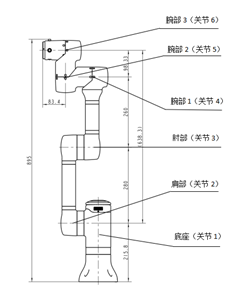
\includegraphics{image/1-1-joints.png}
    \caption{机器人关节示意图}
    \label{fig:机器人关节示意图}
\end{figure}

机器人本体为机器人系统的执行部分,机器人底座为机器人本体安装处,肩部和肘部可执行较大幅度动作,腕部1和腕部 2可执行较精细动作,腕部 3 可以连接末端工具。

控制箱为机器人系统的控制部分,可控制机器人在工作空间中的运动位置、姿态和运行轨迹,连接设备的电气输入和输出端以及机器人的各种状态数据和信息的查看。在实际应用场景下,为确保运行安全,通常需要在控制箱上外接急停开关(选配)。

\begin{figure}[ht]
    \centering
    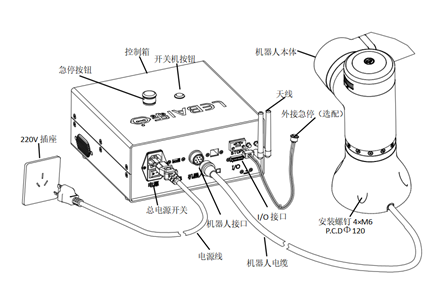
\includegraphics{image/1-2-host.png}
    \caption{机器人本体及控制箱连接示意图}
\end{figure}

机器人控制箱提供 4个数字输入,4个数字输出接口及 2 个模拟输入,2个模拟输出I/O接口;机器人末端法兰盘上提供 2个数字输入,2个数字输出I/O接口。

控制箱通过机器人电缆与机器人本体连接。

\begin{figure}[ht]
    \centering
    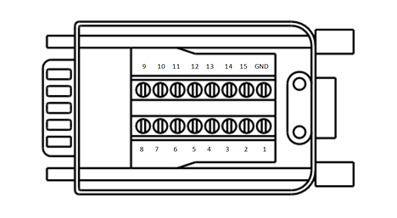
\includegraphics{image/1-3-io.png}
    \caption{I/O硬件接口示意图}
\end{figure}

\begin{table}[ht]
    \centering
\begin{tabularx}{\textwidth}{ccX}
    序号	&   功能	&   性能参数\\\hline
    1	&   电源正极	& 24V  \\
    2	&   模拟输出1   &  
        支持两种输出模式:
        \begin{itemize}
\setlength{\itemsep}{0pt}
\setlength{\topsep}{0pt}
\setlength{\parsep}{0pt}
\setlength{\parskip}{0pt}
            \item 电压型:输出电压信号0~10V;
            \item 电流型:输出电流4~20mA。
        \end{itemize}
    \\
    3	&   模拟输出2 & \\
    4	&   数字输出1	&   输出电压24V,最大电流2A。\\
    5	&   数字输出2	&   \\
    6	&   数字输出3	&   \\
    7	&   数字输出4	&   \\
    8	&   电源负极	&   \\
    9	&   模拟输入1 &   
        支持两种输出模式:
        \begin{itemize}
            \setlength{\itemsep}{0pt}
            \setlength{\topsep}{0pt}
            \setlength{\parsep}{0pt}
            \setlength{\parskip}{0pt}
            \item 电压型:输出电压信号0~10V;
            \item 电流型:输出电流4~20mA。
        \end{itemize}
    \\
    10	&   模拟输入2	&   \\
    11	&   数字输入1	&   输入电压3~30V。\\
    12	&   数字输入2	&   \\
    13	&   数字输入3	&   \\
    14	&   数字输入4	&   \\
    15	&   电源负极	   &     \\
\end{tabularx}
\caption{I/O硬件接口参数表}
\end{table}


用户可通过电脑、平板、手机或其他图形化终端设备的浏览器\footnote{建议使用 Google Chrome 浏览器、Microsoft Edge浏览器或其他基于Webkit 内核的现代浏览器来获得更好的访问质量。}访问机器人示教编程页面进行相关操作。




 
\subsection{底座安装}
如\prettyref{fig:机器人安装方式},LM3机器人支持三种安装方式:正装、倒装、侧装。使用机器人配件包中的 4 颗 M6 螺钉,对应机器人底座上的 4 个螺纹孔进行安装操作,建议以 $9\Nm$ 扭矩紧固这些螺钉。如果需要更准确地调整机器人位置,还可钻2 个直径5 mm的孔,并用销加以固定。
  

\begin{figure}[ht]
    \centering
    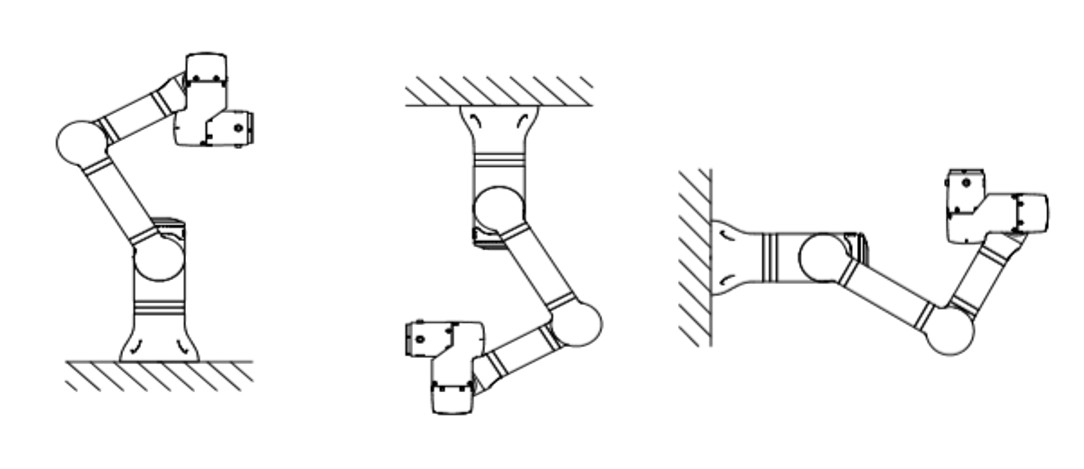
\includegraphics[width=\textwidth]{image/1-4-direction.jpg}
    \caption{机器人安装方式}
    \label{fig:机器人安装方式}
\end{figure}

 
\begin{figure}[ht]
    \centering
    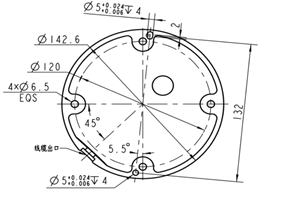
\includegraphics{image/1-5-base.png}
    \caption{机器人底座视图}
    \label{fig:机器人底座视图}
\end{figure}


\info{
机器人每一个孔位都应固定螺钉,固定后的每个螺钉都应能提供最小抗倾覆力。
}



 

 
 
\subsection{末端工具安装}

机器人末端法兰盘正面有4个 M6 螺纹孔,用于连接末端工具与机器人;法兰盘侧面有4个M3螺纹孔,用于乐白轻量化末端工具的安装。正常使用且不包括受外界碰撞情况下,机器人末端(含工具)最大可承受 3 kg负载。



\begin{figure}[ht]
    \centering
    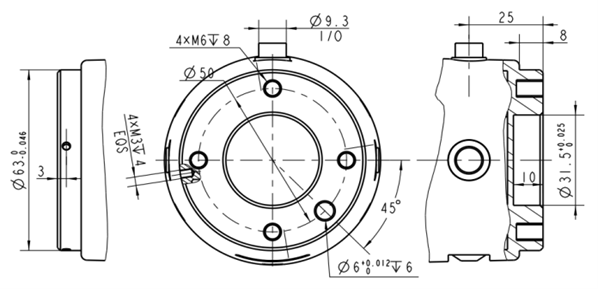
\includegraphics[width=\textwidth]{image/1-6-flange.png}
    \caption{机器人末端法兰盘接口}
    \label{fig:机器人末端法兰盘接口}
\end{figure}
